\subsection{Ordnungsrelationen}\index{Ordnungsrelationen}

\begin{tabular}{c|l}
  $a=b$                        & Gleichheit\noTRAINER{\hspace{20mm}}\\
  $\pi\ne 3$                   & \TNDF{Ungleichheit}\\
  $\pi\approx \frac{355}{113}$ & \TNDF{ungefähr gleich}\\
  $a<b$                        & \TNDF{$a$ ist kleiner als $b$}\\
  $3>1$                        & \TNDF{Analog:  ... ist größer als ...}\\
  $6.022 \cdot{} 10^{-6} \ll 1$ &\TNDF{... sehr viel kleiner als...}\\
  $10^{100} \gg 1000$           & \TNDF{... sehr viel größer als...}\\
  $a\leq b$                    & \TNDF{$a$ kleiner als oder gleich $b$ }\\
  $a\geq 4$                    & \TNDF{Analog: $a$ ist gleich 4 oder größer als 4}  \\
  \hline
\end{tabular}


\subsubsection{Intervall-Notation}

\renewcommand{\arraystretch}3
\begin{tabular}{c|c|c}

  Relation & Zahlenstrahl & Intervallschreibweise \\
  \hline
  $a \geq 4$  &
  \TRAINER{\raisebox{-5mm}{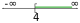
\includegraphics[width=40mm]{allg/alg/img/intervallGE4.png}}}
  \noTRAINER{\hspace{6cm}} & $[4;  \infty [$\\
      \hline
      
  $x\leq 5$ und $x > -2$  &
      \TRAINER{\raisebox{-5mm}{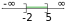
\includegraphics[width=40mm]{allg/alg/img/intervallM2T5.png}}}
      & \TNDF{$]-2; 5]$}\\
  
  \hline
  $-42 > z$  &
  \TRAINER{\raisebox{-5mm}{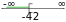
\includegraphics[width=40mm]{allg/alg/img/intervallLE-42.png}}} & \TNDF{$] -\infty ; -42[ $}\\
\hline  
\end{tabular}
\renewcommand{\arraystretch}1
\newpage



\subsection*{Aufgaben zu Ordnungsrelationen}

\aufgabenFarbe{Setzen Sie das richtige Zeichen ($<$, $>$, $=$) zwischen die folgenden Zahlen:}

$\pi \LoesungsRaum{<} \sqrt{10}$ ($\pi$ ist die Kreiszahl)

$-\sqrt{5} \LoesungsRaum{<} \sqrt{2}-\sqrt{13}$

$\frac{10}3 \LoesungsRaum{>} 0.3333333333$

$\e \LoesungsRaum{>} \frac{163}{60}$ ($\e$ ist die Eulersche Zahl)

$8.\overline{9} \LoesungsRaum{=} 18.33 - \frac{933}{100}$

$-\sqrt{6} \LoesungsRaum{\ne} \sqrt{-6}$ \TRAINER{(Fangfrage, denn $\sqrt{-6}$ liegt außerhalb $\mathbb{R}.$)}

\aufgabenFarbe{Ordnen Sie die folgenden Werte der Zahlen bzw. Terme der Reihe nach (auch hier bezeichnet $e$ die Eulersche Zahl):}

$\pi$, $\frac{10}3$, $\sqrt{10}, \sqrt{3^3}-2, (-2.2)\cdot(-1.5), \e+\frac{41}{50}$

\mmPapier{1.6}

\aufgabenFarbe{Welche der folgenden Aussagen sind wahr (auch hier ist $\e$ die Eulersche Zahl)?}

$\pi > \e$ \TRAINER{Wahr}

$\pi = 3.14$ \TRAINER{Falsch}

$\pi = 3.14159265$ \TRAINER{Falsch}

$0.1\overline{6} < \frac16$ \TRAINER{Falsch}

$\e \approx 2.71828$ \TRAINER{Wahr, wenn auch relativ}

$-\sqrt{3} < 0 - \sqrt{2}$ \TRAINER{Wahr}

$\sqrt{\frac{8^8}{\e\cdot{}\pi}} > 1.9646 \cdot{} 10^6$ \TRAINER{Wahr}



\TNTeop{}

%%\GESOAadB{22f}{10. b) 11. a) b) c) d)}
%%\TALSAadB{13}{13.}
%%\TRAINER{Spätestens hier auf die Musterlösungswege im OLAT hinweisen.}
